\documentclass[tikz, border=1pt]{standalone}
\pdfoutput=1 % if your are submitting a pdflatex (i.e. if you have
             % images in pdf, png or jpg format)

\usepackage{graphicx}

% Use the tikz package
\usepackage{tikz}
\usetikzlibrary{decorations}


\begin{document}

        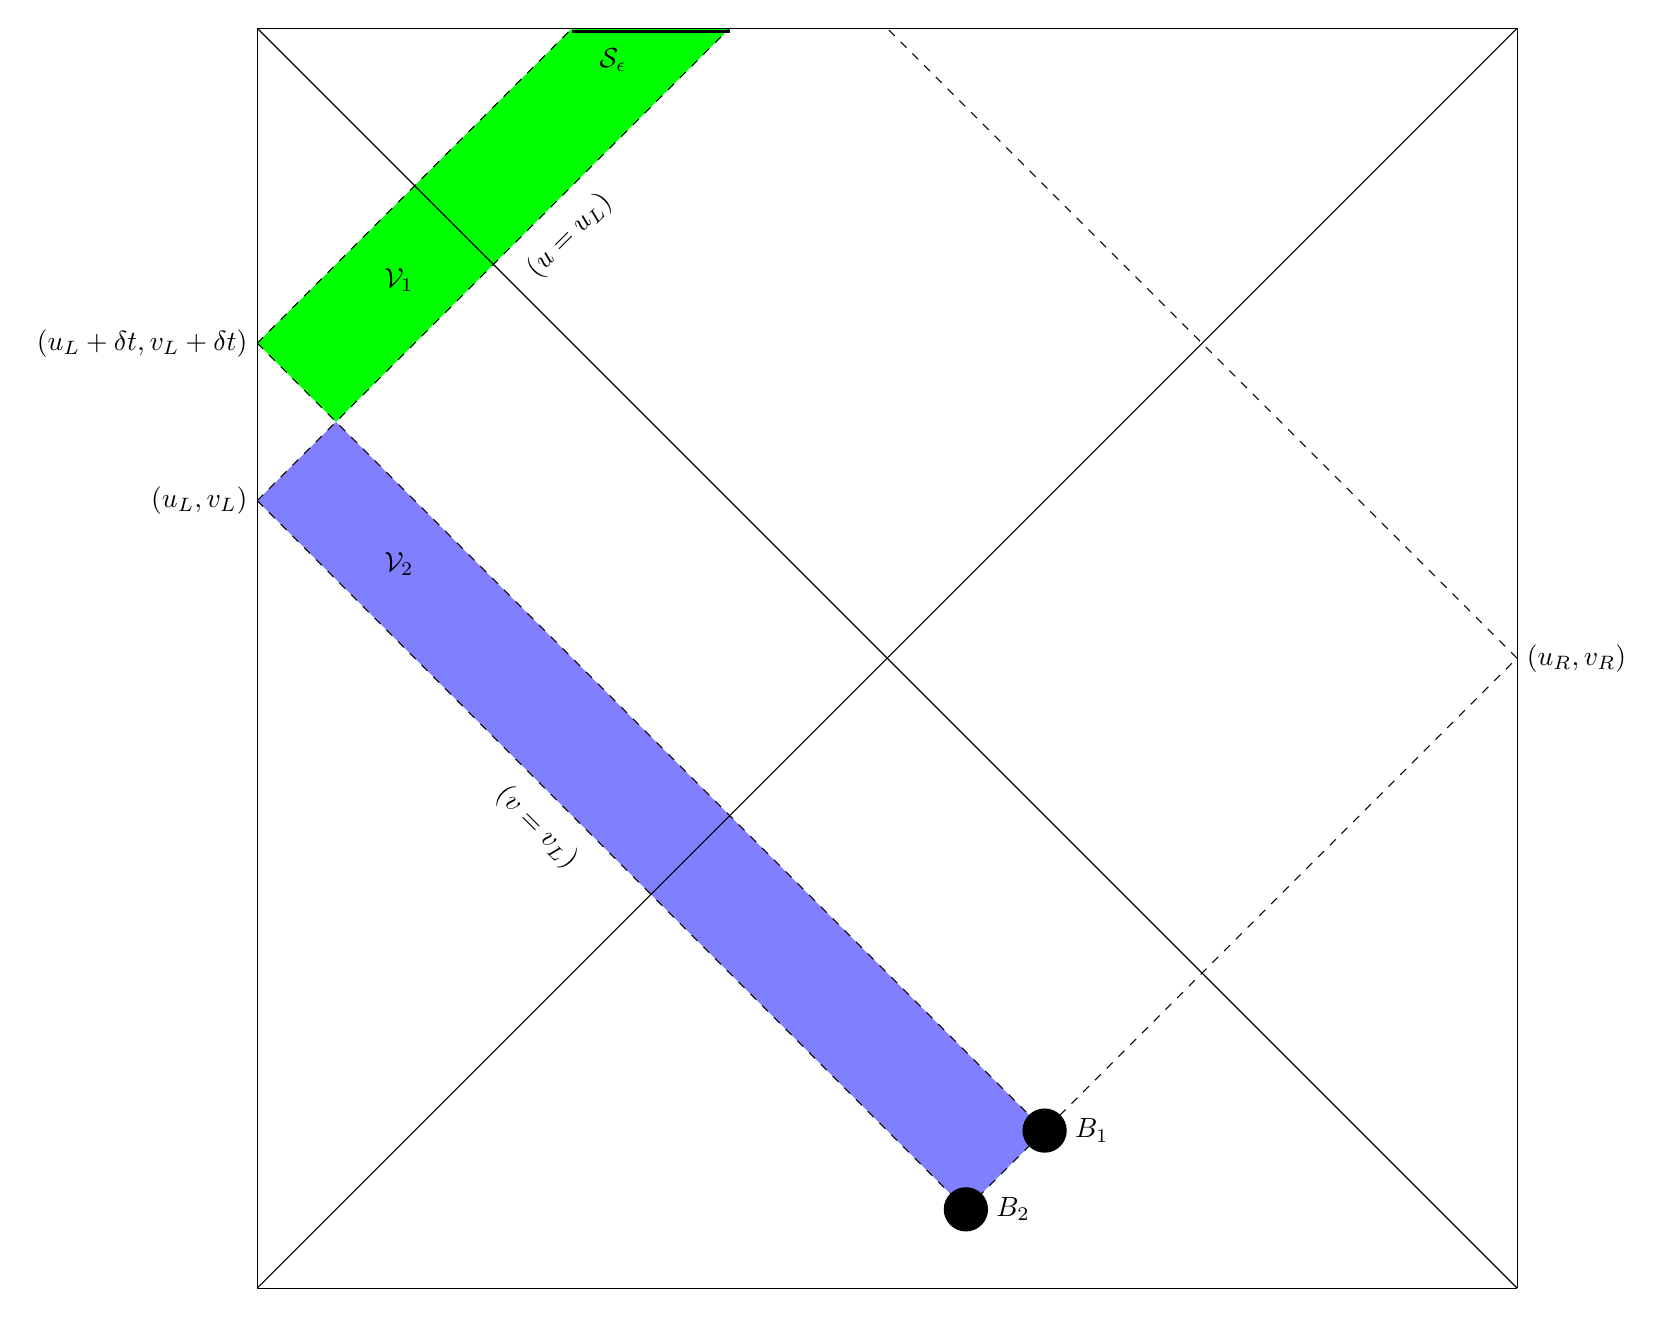
\begin{tikzpicture}[scale=4]
        
        % Shade bulk regions
        \fill[green] (0.25,2.75)--(0,3)--(1,4)--(1.5,4)--(0.25,2.75);
        \fill[blue!50!white] (0.25,2.75)--(0,2.5)--(2.25,0.25)--(2.5,0.5)--(0.25,2.75);
        
        % WdW boundaries
        \draw[dashed] (0,3)--(1,4);
        \draw[very thick] (1,3.99)--(1.5,3.99);
        \draw[dashed] (0,2.5)--(1.5,4); 
        \draw[dashed] (0,3)--(2.5,.5); 
        \draw[dashed] (0,2.5)--(2.25,.25);
        \draw[dashed] (2.25,.25)--(4,2);
        \draw[dashed] (4,2)--(2,4);
        
        %axes
        \draw (0,0)--(4,0);
        \draw (4,0) --(4,4);
        \draw (4,4)--(0,4);
        \draw (0,4)--(0,0);
        \draw (0,0) --(4,4);
        \draw (0,4)--(4,0);
        
        %\fill(.25,2.75) circle[radius=2pt];
        \fill(2.5,.5) circle[radius=2pt];
        \fill(2.25,.25) circle[radius=2pt];
        
        %labels
        \draw (0.45,3.2) node{$\mathcal{V}_1$};
        \draw (0.45,2.3) node{$\mathcal{V}_2$};
        \draw (2.4,.25) node{$B_2$};
        \draw (2.65,.5) node{$B_1$};
        \draw (1.13,3.9) node{$\mathcal{S}_\epsilon$};
        \draw (0,2.5) node[left]{$(u_L,v_L)$};
        \draw (0,3) node[left]{$(u_L+\delta t,v_L + \delta t)$};
        \draw (4,2) node[right]{$(u_R,v_R)$};
        \draw (.75,1.6) node[right, rotate=-45]{$(v=v_L)$};
        \draw (.85,3.2) node[right, rotate=45]{$(u=u_L)$};
        \end{tikzpicture}

\end{document}
